%!TEX program = xelatex
%!TEX spellcheck = en_GB
\documentclass[final]{article}
% Include all project wide packages here.
%\usepackage{fullpage}
\usepackage[a4paper,margin=2.5cm,top=2cm]{geometry}
\usepackage{polyglossia}
\setmainlanguage{english}
\usepackage{csquotes}
\usepackage{graphicx}
\usepackage{pdfpages}
\usepackage{caption}
\usepackage[list=true]{subcaption}
\usepackage{float}
\usepackage{standalone}
\usepackage{import}
\usepackage{tocloft}
\usepackage{wrapfig}
\usepackage{authblk}
\usepackage{array}
\usepackage{booktabs}
\usepackage[title,titletoc]{appendix}
\usepackage{fontspec}
\usepackage{pgfplots}
\usepackage{tikz}
\usepackage[binary-units=true,table-auto-round]{siunitx}
\usepackage{units}
\usepackage{amsmath}
\usepackage{mathtools}
\usepackage{unicode-math}
\usepackage{rotating}
\usepackage{titlesec}
\usepackage{titletoc}
\usepackage{blindtext}
\usepackage{color}
\usepackage{enumitem}
\usepackage{tabularx}
\usepackage{titling}
\usepackage{multirow}
\usepackage[%
siunitx,
fulldiodes,
europeanvoltages,
europeancurrents,
europeanresistors,
americaninductors,
smartlabels]{circuitikz}

\newcommand{\matlab}{{\textsc{matlab }}}

\usetikzlibrary{calc}
\usetikzlibrary{positioning}
\usetikzlibrary{automata}
\usetikzlibrary{arrows.meta}

\tikzstyle{every state}=[fill=tu-cyan,align=center,draw=black,line width=1pt,node distance=3cm,minimum width = 1.8cm]%for FSMs casper
\tikzstyle{every initial by arrow}=[initial text={Reset}]
\newcommand{\setpathasarrows}{\tikzstyle{every path}=[auto,line width=1.5pt,line cap=round,line join=round]}

\pgfplotsset{compat=newest}
\pgfplotsset{plot coordinates/math parser=false}
\usetikzlibrary{plotmarks}
\usepgfplotslibrary{patchplots}
\newlength\figureheight
\newlength\figurewidth

\tikzset{every axis/.style={xticklabel style={align=right}}}

\usepackage[
%backend=bibtex,
backend=biber,
	texencoding=utf8,
    bibencoding=utf8,
    style=numeric,
    citestyle=numeric,
    sortlocale=en_US,
    language=auto,
    backref=true,
    abbreviate=false,
    date=edtf,
    seconds=true
]{biblatex}

\usepackage{listings}
\newcommand{\includecode}[4][c]{\lstinputlisting[caption=#2, escapechar=, style=#1,label=#4]{#3}}
\newcommand{\superscript}[1]{\ensuremath{^{\textrm{#1}}}}
\newcommand{\subscript}[1]{\ensuremath{_{\textrm{#1}}}}


\newcommand{\chapternumber}{\thechapter}
\renewcommand{\appendixname}{Appendix}
\renewcommand{\appendixtocname}{Appendices}
\renewcommand{\appendixpagename}{Appendices}


\setlist[enumerate]{labelsep=*, leftmargin=1.5pc}
\setlist[enumerate,1]{label=\arabic*., ref=\arabic*}
\setlist[enumerate,2]{label=\arabic*.,ref=\theenumi.\arabic*}
\setlist[enumerate,3]{label=\arabic*., ref=\theenumii.\arabic*}

%\setcounter{chapter}{-1} %start chapter numbers with 0

\usepackage{xr-hyper}
\usepackage[hidelinks]{hyperref} %<--------ALTIJD ALS LAATSTE
\usepackage[nameinlink,noabbrev,capitalise]{cleveref} %<------- Clever Ref moet na hyperref
\crefname{app}{Appendix}{Appendices}
%\renewcommand{\familydefault}{\sfdefault}


\setmainfont{Myriad Pro}[Ligatures={Common,TeX}]
%\setmathfont{Asana Math}
\setmathfont{Asana-Math.otf}
\setmonofont[Scale=0.9]{Lucida Console}
\newfontfamily\headingfont{Minion Pro}[Ligatures={Common,TeX}]


%Design colors
\definecolor{accent1}{RGB}{0,100,200}
\definecolor{accent2}{RGB}{0,50,100}
\definecolor{tu-cyan}{RGB}{0,166,214}

\newcommand{\hsp}{\hspace{20pt}}
% \titleformat{\chapter}[hang]{\Huge\headingfont}{\chapternumber\hsp\textcolor{accent2}{|}\hsp}{0pt}{\Huge\headingfont}

% \titleformat{name=\chapter,numberless}[hang]{\Huge\headingfont}{\hsp\textcolor{accent2}{|}\hsp}{0pt}{\Huge\headingfont}

% \titleformat{\section}[block]{\LARGE\headingfont}{\arabic{chapter}.\arabic{section}}{0.4em}{}
% \titleformat{\subsection}[block]{\Large\headingfont}{\arabic{chapter}.\arabic{section}.\arabic{subsection}}{0.4em}{}
% \titleformat{\subsubsection}[block]{\large\headingfont}{\arabic{chapter}.\arabic{section}.\arabic{subsection}.\arabic{subsubsection}}{0.4em}{}
\renewcommand{\arraystretch}{1.2}
\renewcommand{\baselinestretch}{1.25} 

\renewcommand\cfttoctitlefont{\headingfont\Huge}
\renewcommand\cftloftitlefont{\headingfont\Huge}
\renewcommand\cftlottitlefont{\headingfont\Huge}
\setcounter{lofdepth}{2}
\setcounter{lotdepth}{2}


\setlength{\parindent}{0pt}
\setlength{\parskip}{1em}

\captionsetup{width=0.9\textwidth}

%SIuntix settings:
%default: 0V to 10V
%custom: 0 - 10V
\sisetup{range-phrase=--}
\sisetup{range-units=single}
\DeclareSIUnit\years{years}

%For code listings
\definecolor{black}{rgb}{0,0,0}
\definecolor{browntags}{rgb}{0.65,0.1,0.1}
\definecolor{bluestrings}{rgb}{0,0,1}
\definecolor{graycomments}{rgb}{0.4,0.4,0.4}
\definecolor{redkeywords}{rgb}{1,0,0}
\definecolor{bluekeywords}{rgb}{0.13,0.13,0.8}
\definecolor{greencomments}{rgb}{0,0.5,0}
\definecolor{redstrings}{rgb}{0.9,0,0}
\definecolor{purpleidentifiers}{rgb}{0.01,0,0.01}


\lstdefinestyle{csharp}{
language=[Sharp]C,
showspaces=false,
showtabs=false,
breaklines=true,
showstringspaces=false,
breakatwhitespace=true,
escapeinside={(*@}{@*)},
columns=fullflexible,
commentstyle=\color{greencomments},
keywordstyle=\color{bluekeywords}\bfseries,
stringstyle=\color{redstrings},
identifierstyle=\color{purpleidentifiers},
basicstyle=\ttfamily\small}

\lstdefinestyle{c}{
language=C,
showspaces=false,
showtabs=false,
breaklines=true,
showstringspaces=false,
breakatwhitespace=true,
escapeinside={(*@}{@*)},
columns=fullflexible,
commentstyle=\color{greencomments},
keywordstyle=\color{bluekeywords}\bfseries,
stringstyle=\color{redstrings},
identifierstyle=\color{purpleidentifiers},
}

\lstdefinestyle{matlab}{
language=Matlab,
showspaces=false,
showtabs=false,
breaklines=true,
showstringspaces=false,
breakatwhitespace=true,
escapeinside={(*@}{@*)},
columns=fullflexible,
commentstyle=\color{greencomments},
keywordstyle=\color{bluekeywords}\bfseries,
stringstyle=\color{redstrings},
identifierstyle=\color{purpleidentifiers}
}

\lstdefinestyle{vhdl}{
language=VHDL,
showspaces=false,
showtabs=false,
breaklines=true,
showstringspaces=false,
breakatwhitespace=true,
escapeinside={(*@}{@*)},
columns=fullflexible,
commentstyle=\color{greencomments},
keywordstyle=\color{bluekeywords}\bfseries,
stringstyle=\color{redstrings},
identifierstyle=\color{purpleidentifiers}
}

\lstdefinestyle{xaml}{
language=XML,
showspaces=false,
showtabs=false,
breaklines=true,
showstringspaces=false,
breakatwhitespace=true,
escapeinside={(*@}{@*)},
columns=fullflexible,
commentstyle=\color{greencomments},
keywordstyle=\color{redkeywords},
stringstyle=\color{bluestrings},
tagstyle=\color{browntags},
morestring=[b]",
  morecomment=[s]{<?}{?>},
  morekeywords={xmlns,version,typex:AsyncRecords,x:Arguments,x:Boolean,x:Byte,x:Char,x:Class,x:ClassAttributes,x:ClassModifier,x:Code,x:ConnectionId,x:Decimal,x:Double,x:FactoryMethod,x:FieldModifier,x:Int16,x:Int32,x:Int64,x:Key,x:Members,x:Name,x:Object,x:Property,x:Shared,x:Single,x:String,x:Subclass,x:SynchronousMode,x:TimeSpan,x:TypeArguments,x:Uid,x:Uri,x:XData,Grid.Column,Grid.ColumnSpan,Click,ClipToBounds,Content,DropDownOpened,FontSize,Foreground,Header,Height,HorizontalAlignment,HorizontalContentAlignment,IsCancel,IsDefault,IsEnabled,IsSelected,Margin,MinHeight,MinWidth,Padding,SnapsToDevicePixels,Target,TextWrapping,Title,VerticalAlignment,VerticalContentAlignment,Width,WindowStartupLocation,Binding,Mode,OneWay,xmlns:x}
}

\lstdefinestyle{python}{
language=Python,
showspaces=false,
showtabs=false,
breaklines=true,
showstringspaces=false,
breakatwhitespace=true,
escapeinside={(*@}{@*)},
columns=fullflexible,
commentstyle=\color{greencomments},
keywordstyle=\color{bluekeywords}\bfseries,
stringstyle=\color{redstrings},
identifierstyle=\color{purpleidentifiers},
}

%defaults
\lstset{
basicstyle=\ttfamily\scriptsize ,
extendedchars=false,
numbers=left,
numberstyle=\ttfamily\tiny,
stepnumber=1,
tabsize=4,
numbersep=5pt
}
\addbibresource{../../.library/bibliography.bib}
\begin{document}

%TODO make macros for all the $A_{blah}$ specifiers. These look bad. They should be SIunitsx units and not italic.
\section{Performance Evaluation}
\label{sec:performance-eval}
As part of the midterm milestone meeting the baseline performance of the processor was re-evaluated.
After that the size of the cache was increased and the cache mapping mechanism was improved to give it the ability to cache the full \SI{4}{\mega\byte} of the main memory.
This section discusses the results of these experiments.

\subsection{Baseline}
\Cref{tab:baselinebench,tab:baselineperformance} show a comparison of reported performance versus measured performance. All the benchmarks were run on the FPGA to obtain the measured benchmark scores of \cref{tab:baselinebench}. The opcodes benchmark was simulated using QuestaSim. All the measured benchmarks are close to those reported in the project manual.
\begin{table}[H]
    \centering
    \caption{Comparison of benchmark scores reported by project manual and measured benchmark scores. All scores in million cycles.}
    \label{tab:baselinebench}
    \begin{tabular}{lS[table-format=1.6]S[table-format=1.6]}
        \toprule
        \textbf{Name}       & \textbf{Benchmark score (reported)} & \textbf{Benchmark score (measured)} \\
        \midrule
        opcodes    & \textrm{verified}          & \textrm{verified}                     \\
        cjpeg      & 29.740140                  & 29.316406                             \\
        divide     & 264.820001                 & 274.860369                            \\
        multiply   & 149.492876                 &   155.283095                          \\
        pi         & 845.277552                 &   845.294532                          \\
        fir        & 187.411039                 &  187.537571                           \\
        rsa        & 563.89053                  &   577.504991                          \\
        ssd        & 797.170350                 &  860.871400                           \\
        ssearch    & 457.727967                 &  475.458147                           \\
        susan      & 910.498879                 &  916.969617                           \\
        bench\_all & 4323.096258                &  4323.096128                          \\
        \bottomrule
    \end{tabular}
\end{table}

For \cref{tab:baselineperformance} the steps from the project manual were followed to generate the specifications.
For area 9 $A_{FIFO16/RAMB16}$ and 2022 $A_{SLICE}$ were found which resulted in an area of 514.5 $A_{CLB}$ when the weights of $A_{FIFO16/RAMB16} = A_{CLB}$ and $A_{SLICE} = A_{CLB}/4$ from the project manual were used.
For frequency the minimum clock period was found to be \SI{23.686}{\nano\second} which resulted in \SI{42.219}{\mega\hertz} as the maximum frequency.
Power was estimated for the pi benchmark with \SI{1}{\milli\second} simulation time which resulted in a total power estimate of \SI{0.698}{\watt}.
A more detailed power analysis can be found in \cref{fig:baselinepower}
The power, area and frequency totals are all equal to those reported in the project manual.
The more detailed power analysis in \cref{fig:baselinepower} is not exactly the same but very similar to the values found in the manual.

%TODO make table with S[table-format=1.6] (for the numbers) and s (for the units columns) This will work after the TODO at the top of this page is done. So it will look like this: lS[table-format=2.3]sS[table-format=2.3]s
\begin{table}[H]
    \centering
    \caption{Comparison of baseline specifications reported by project manual and measured specifications.}
    \label{tab:baselineperformance}
    \begin{tabular}{lll}
        \toprule
        \textbf{Attribute} & \textbf{Reported} & \textbf{Measured} \\
        \midrule
        Power    &  \SI{0.698}{\watt}        &   \SI{0.698}{\watt}                \\
        Area     &       \num{541.5} $A_{CLB}$            & \num{541.5} $A_{CLB}$             \\
        Frequency    &   \SI{42.219}{\mega\hertz}           &  \SI{42.219}{\mega\hertz}                         \\
        \bottomrule
    \end{tabular}

\end{table}

%TODO Make into proper image. This screenshot looks like shit.
\begin{figure}[H]
\centering
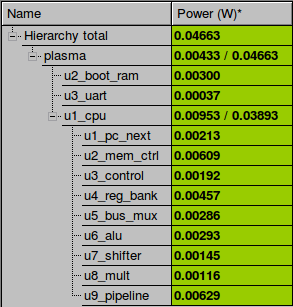
\includegraphics[width=0.3\textwidth]{resources/baselinepower.png}
\caption{Detailed power analysis by hierarchy for baseline processor.}
\label{fig:baselinepower}
\end{figure}

\subsection{Larger cache}
For the first attempt at improving the speed of the processor the size of the cache was enlarged as dictated by the milestone meeting goals.
The default Plasma processor only utilized half of 4 implemented \SI{2}{\kibi\byte} memory blocks so increasing the cache to \SI{8}{\kibi\byte} could be done without increasing the area footprint of the design.
For the \SI{16}{\kibi\byte} design 5 extra \SI{2}{\kibi\byte} memory blocks were needed to accommodate not only the extra \SI{8}{\kibi\byte} worth of cache memory but also an extra \SI{2}{\kibi\byte} block for storing cache tags.
This increases the area foot print of the \SI{16}{\kibi\byte} design with 5 $A_{FIFO16/RAMB16}$.
The results of the benchmarks for the new designs can be found in \cref{tab:largecachebench}.
A decrease in clock cycles needed can definitely be observed.
The \SI{8}{\kibi\byte} design sees an improvement of $1.79\%$ while the \SI{16}{\kibi\byte} design improves $4.33\%$ in respect to the \SI{4}{\kibi\byte} cache.
\begin{table}[H]
    \centering
    \caption{Comparison of benchmark scores reported by project manual and measured benchmark scores. All scores in million cycles.}
    \label{tab:largecachebench}
    \begin{tabular}{lS[table-format=1.6]S[table-format=1.6]S[table-format=1.6]}
        \toprule
        \textbf{Name}        & \textbf{\SI{4}{\kibi\byte}} & \textbf{\SI{8}{\kibi\byte}} & \textbf{\SI{16}{\kibi\byte}} \\
        \midrule
        cjpeg       & 29.316406                 & 28.455434               &   27.842593        \\
        divide      & 274.860369                & 265.116735               &  255.882408          \\
        multiply    &   155.283095              & 150.094662               &  145.348008          \\
        pi          &   845.294532              &  844.614099              &  843.899086          \\
        fir         &  187.537571               &  186.518289               & 185.996077           \\
        rsa         &   577.504991              &  574.562761               & 570.101571           \\
        ssd         &  860.871400               & 833.108159                & 745.625121           \\
        ssearch     &  475.458147               &  448.907365               & 448.906471           \\
        susan       &  916.969617               & 914.132525                &  912.359250          \\
        bench\_all  &  4323.096128              & 4245.510029               &  4135.960585          \\
        \bottomrule
    \end{tabular}

\end{table}


\subsection{Improved cache mapping}
\end{document}